% Tiny contract
% Teams: Suspension
% Requirements: REQ-DES-130 REQ-FUN-020
% Status: [done]
\begin{figure}[H]
\centering
\captionsetup{font=footnotesize}
\captionsetup[subfigure]{font=footnotesize}

\begin{minipage}{0.78\textwidth}
\centering

\begin{subfigure}[t]{0.49\linewidth}
\centering
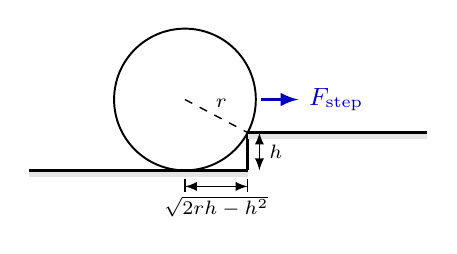
\begin{tikzpicture}[scale=6, >=latex]

  %% ---- Parameters ----
  \pgfmathsetmacro{\rr}{0.15}
  \pgfmathsetmacro{\hh}{0.08}

  %% ---- Derived ----
  \pgfmathsetmacro{\cx}{sqrt(2*\rr*\hh - \hh*\hh)}

  %% ---- Lower ground (left) ----
  \fill[gray!20] ({-\cx-\rr-0.18}, {-0.013}) rectangle (0, 0);
  \draw[line width=1.0pt] ({-\cx-\rr-0.18}, 0) -- (0, 0);

  %% ---- Step vertical face ----
  \draw[line width=1.0pt] (0, 0) -- (0, {\hh});

  %% ---- Upper ground (right) ----
  \fill[gray!20] (0, {\hh-0.013}) rectangle (0.38, {\hh});
  \draw[line width=1.0pt] (0, {\hh}) -- (0.38, {\hh});

  %% ---- Wheel ----
  \draw[line width=0.7pt] ({-\cx}, {\rr}) circle (\rr);

  %% ---- r: dashed line, label shifted above-left clear of circle stroke ----
  \draw[dashed, line width=0.5pt]
    ({-\cx}, {\rr}) -- (0, {\hh});
  \node[font=\scriptsize] at ({-\cx*0.42}, {\rr + (\hh-\rr)*0.42 + 0.022})
    {$r$};

  %% ---- h: vertical arrow right of step face ----
  \draw[latex-latex, line width=0.5pt]
    (0.025, 0) -- (0.025, {\hh})
    node[midway, right, font=\scriptsize] {$h$};

  %% ---- sqrt(2rh-h^2): horizontal arrow below lower ground ----
  \draw[latex-latex, line width=0.5pt]
    ({-\cx}, {-0.034}) -- (0, {-0.034})
    node[midway, below, font=\scriptsize] {$\sqrt{2rh - h^2}$};
  \draw[line width=0.4pt] ({-\cx}, {-0.018}) -- ({-\cx}, {-0.046});
  \draw[line width=0.4pt] (0,      {-0.018}) -- (0,      {-0.046});

  %% ---- F_step arrow ----
  \draw[->, line width=1.2pt, blue!75!black]
    ({-\cx+\rr+0.012}, {\rr})
    -- ({-\cx+\rr+0.09}, {\rr})
    node[right, font=\small\bfseries] {$F_{\mathrm{step}}$};

\end{tikzpicture}
\caption{Step-climbing geometry with obstacle height $h$ and wheel radius $r$.}
\label{fig:step_geom}
<<<<<<< des/2_1_3_wheel_design
\vspace{-0.5\baselineskip}
\end{wrapfigure}

Drive motor selection was based on two parallel analyses.
First, a traction model accounting for rover mass, rolling
resistance of Mars~yard terrain, and a \ang{15} slope yields
a required wheel torque of approximately \SI{12}{\newton\metre}
per wheel at \SI{1}{\metre\per\second} with \SI{1}{\second}
acceleration time. Applying a safety factor of $k_s = 1.5$ and
assuming drivetrain efficiency of $\eta = 0.8$ gives a rated
motor requirement of approximately \SI{23.8}{\newton\metre}.
Second, a step-climbing torque analysis was performed, relating
required wheel torque to obstacle height for a wheel radius of
\SI{150}{\milli\metre}; this sets an upper bound of approximately
\SI{40}{\newton\metre} for the maximum obstacle height of
$h^* \approx \SI{127}{\milli\metre}$ (${\approx}\,85\%$ of wheel
radius). Based on these results, the \mbox{DM-J10010L-2EC} hub
motor was selected, providing \SI{40}{\newton\metre} nominal and
\SI{120}{\newton\metre} peak torque at \SI{48}{\volt} ---
satisfying both the traction and obstacle-climbing requirements
with adequate margin. To simplify logistics and electronics
development, the same motor model is used for wheel drive and the shoulder joints of the
manipulator arm.
=======
\end{subfigure}\hfill
\begin{subfigure}[t]{0.49\linewidth}
\centering
\begin{tikzpicture}[scale=0.82, >=Stealth]
  % Slope and horizontal reference
  \draw[gray!60, dashed] (-0.4,0) -- (5.0,0);
  \draw[line width=1.0pt] (0,0) -- ({4.8*cos(15)},{4.8*sin(15)});

  % Wheel geometry on slope
  \pgfmathsetmacro{\rw}{0.55}
  \coordinate (P) at ({2.0*cos(15)},{2.0*sin(15)});
  \coordinate (C) at ({2.0*cos(15)-\rw*sin(15)},{2.0*sin(15)+\rw*cos(15)});
  \draw[line width=0.9pt] (C) circle (\rw);
  \fill (C) circle (1.1pt);

  % Velocity vector uphill (Formula 1 case)
  \draw[->, line width=1.1pt, blue!75!black]
    (C) -- ++({1.15*cos(15)},{1.15*sin(15)})
    node[above right, font=\scriptsize] {$v=\SI{1}{\metre\per\second}$};

  % Weight vector
  \draw[->, line width=0.9pt, red!70!black]
    (C) -- ++(0,-1.0)
    node[right, font=\scriptsize] {$mg$};

  % Slope angle label
  \draw[->, line width=0.6pt] (0.95,0) arc[start angle=0, end angle=15, radius=0.95];
  \node[font=\scriptsize] at (0.82,-0.12) {$\alpha=\ang{15}$};
\end{tikzpicture}
\caption{Uphill case from Formula~1: \ang{15} slope and $v=\SI{1}{\metre\per\second}$.}
\label{fig:uphill_motion_formula1}
\end{subfigure}
\end{minipage}

\caption{Locomotion load cases used for drivetrain sizing.}
\label{fig:locomotion_load_cases}
\end{figure}

Drivetrain torque sizing is based on two governing load cases: uphill traction and step climbing.

All calculations in this subsection are approximate engineering estimates used for system-level sizing, with conservative margin applied in final actuator requirements.

\begin{itemize}[leftmargin=1.2em, itemsep=0.2em, topsep=0.3em]
  \item \textbf{Traction case (\ang{15} slope):} estimated wheel torque
  $\tau_\mathrm{wheel}\approx\SI{12.7}{\newton\metre}$ at
  $v=\SI{1}{\metre\per\second}$ and
  $a=\SI{1}{\metre\per\second\squared}$.

  \item \textbf{Rated motor requirement:} with safety factor
  $k_s=1.5$ and drivetrain efficiency $\eta=0.8$,
  $\tau_\mathrm{rated}\approx\SI{23.8}{\newton\metre}$.

  \item \textbf{Step-climbing case:} for wheel radius
  $r=\SI{150}{\milli\metre}$, the nominal torque limit
  $\SI{40}{\newton\metre}$ corresponds to
  $h^*\approx\SI{127}{\milli\metre}\;(\approx0.85r)$.

  \item \textbf{Motor selection:} \textit{Drive Motor},
  with \SI{40}{\newton\metre} nominal and
  \SI{120}{\newton\metre} peak capability at 48~V,
  covering both load cases with margin.

  \item \textbf{Standardization:} the same motor class is used for
  wheel drive, steering rotation, and manipulator shoulder joints.
\end{itemize}
>>>>>>> main


\begin{table}[h!]
\centering
\caption{Drive motor torque requirements (\(r = \SI{150}{\milli\metre}\), \(m = \SI{75}{\kilo\gram}\), \(N{=}4\) wheels)}
\label{tab:motor_torque}
\setlength{\tabcolsep}{8pt}
\begin{tabular}{@{}llll@{}}
\toprule
\textbf{Load case} & \textbf{Expression} & \textbf{Value} & \textbf{Note} \\
\midrule
\multicolumn{4}{@{}l}{\textit{Traction model}} \\[2pt]
Rolling resistance
  & $F_\mathrm{roll} = C_{rr}\,mg$
  & \SI{73.6}{\newton}
  & $C_{rr}=0.10$ \\
Grade force
  & $F_\mathrm{grade} = mg\sin\alpha$
  & \SI{190.4}{\newton}
  & $\alpha=\ang{15}$ \\
Acceleration force
  & $F_\mathrm{acc} = ma$
  & \SI{75.0}{\newton}
  & $a=\SI{1}{\metre\per\second\squared}$ \\
Total traction force
  & $F_\mathrm{tot} = F_\mathrm{acc}+F_\mathrm{roll}+F_\mathrm{grade}$
  & \SI{339.0}{\newton}
  & \\
Wheel torque
  & $\tau_\mathrm{wheel} = F_\mathrm{tot}\,r/N$
  & \SI{12.7}{\newton\metre}
  & per wheel \\
\textbf{Rated requirement}
  & $\tau_\mathrm{rated} = \tau_\mathrm{wheel}\,k_s/\eta$
  & \textbf{\SI{23.8}{\newton\metre}}
  & $k_s{=}1.5,\;\eta{=}0.8$ \\[4pt]
\multicolumn{4}{@{}l}{\textit{Step-climbing model}} \\[2pt]
Front wheel load
  & $W_\mathrm{front} = mg/N$
  & \SI{183.9}{\newton}
  & 50\,\% front share, 2 wheels \\
Step torque
  & $\tau_\mathrm{step}(h)
    = W_\mathrm{front}\,r\,\dfrac{\sqrt{2rh-h^2}}{r-h}$
  & ---
  & \\
Max obstacle (nominal)
  & $\tau_\mathrm{step}(h^*) = \SI{40}{\newton\metre}$
  & $h^* \approx \SI{127}{\milli\metre}$
  & $0.85\,r$ \\
Max obstacle (peak)
  & $\tau_\mathrm{step}(h^{**}) = \SI{120}{\newton\metre}$
  & $h^{**} \approx \SI{148}{\milli\metre}$
  & $0.99\,r$ \\
\bottomrule
\end{tabular}
\end{table}